% HW02.tex
% Second Homework -- Math 221H
% 
% The percent sign is a comment character
% 
%%%%%%%%%%%%%%%%%%%%%%%%%%%%%%%%%%%%%%%%%%%%%%%%%%%%%%%%%%%%%%%%%%%%%%%%%%%%%%%%%% 
% 
% Look these up on line.  The first sets the type of document, and the next are for mathematics symbols, graphics and color
% 
\documentclass[10pt]{article}
\usepackage{amssymb,amsmath}
\usepackage{graphicx}
\usepackage{mathtools}
\usepackage[usenames,dvipsnames,svgnames,table]{xcolor}
\usepackage{multirow}   % This is for more control over tables
%%%%%%%%%%%%%%%%%%%%%%%%%%%%%%%% Layout     %%%%%%%%%%%%%%%%%%%%%%%%%%%%%%%%%%%%%%
\usepackage{vmargin}
\setpapersize{USletter}
\setmargrb{2cm}{1cm}{2cm}{1cm} % --- sets all four margins LTRB


\newcommand{\RR}{{\mathbb R}}  % This is the backboard bold symbol for the real numbers.  Note how it is used below
\newcommand{\NN}{{\mathbb N}}  % 
\newcommand{\ZZ}{{\mathbb Z}}  %

\newcommand{\calP}{{\mathcal P}}  %Caligraphic P for power set

\newcommand{\bfa}{{\bf a}}    %Vectors
\newcommand{\bfb}{{\bf b}}    %Vectors
\newcommand{\bfc}{{\bf c}}    %Vectors
\newcommand{\bfd}{{\bf d}}    %Vectors
\newcommand{\bfv}{{\bf v}}    %Vectors
\newcommand{\bfw}{{\bf w}}    %Vectors
\newcommand{\bfi}{{\bf i}}    %Unit Vectors
\newcommand{\bfj}{{\bf j}}    %Unit Vectors
\newcommand{\bfk}{{\bf k}}    %Unit Vectors

\newcommand{\sep}{{\ :\ }}     % This is for the : in our notation for building sets.
% an acceptable (and common) alternative is \mid  (try it!)

\graphicspath{ {./} }

%%%%%%%%%%%%%%%%%%%%%%%%%%%%%%%%%%%%%%%%%%%%%%%%%%%%%%%%%%%%%%%%%%%%%%%%%%%%%%%%% 
\begin{document}
\LARGE 
\noindent
{\color{Maroon}Lab Report 4}\vspace{2pt}
\hfill \Large Seungheon Oh\vspace{2pt}

\begin{align*}
  p &= v * m & E &= \frac{1}{2}mv^2 = \frac{1}{2}m(v_{ax}^2+v_{ay}^2)\\
  P&= \bar{P} + \delta P & E &= \bar{E} + \delta E \\
  \bar{P_x} &= \bar{P_{Ax}} + \bar{P_{Bx}} & \delta E &= \sqrt{\delta E_a^2+\delta E_b^2}\\
  \delta P_x &= \sqrt{\delta P_{Ax}^2 + \delta P_{Bx}^2}
\end{align*}

\begin{center}
  \makebox[\textwidth]{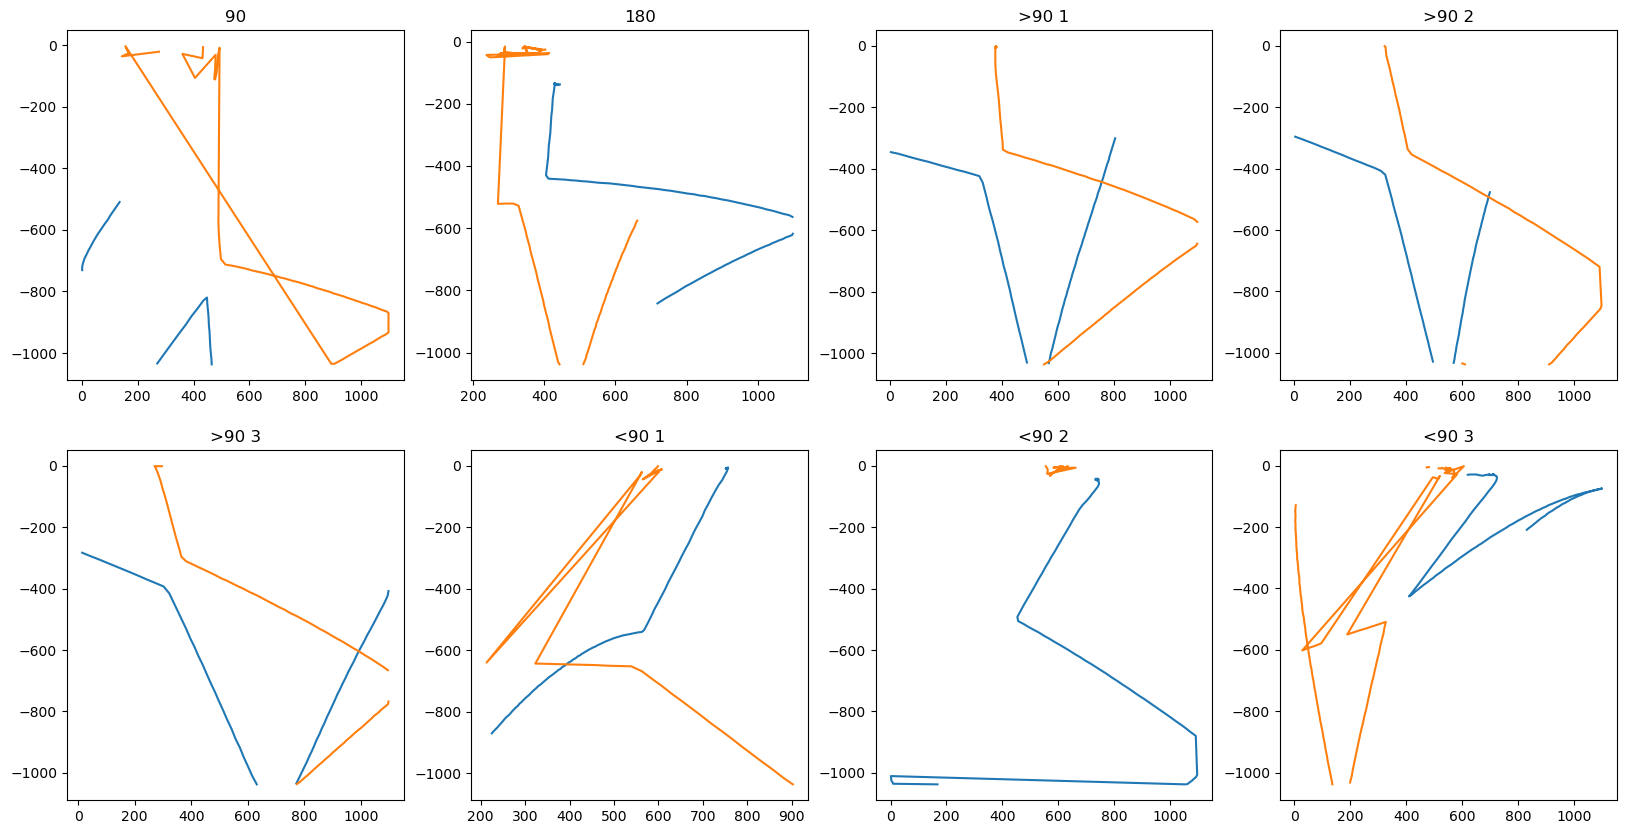
\includegraphics[width=\paperwidth]{1}}
\end{center}

\normalsize

\end{document}

%%% Local Variables:
%%% mode: latex
%%% TeX-master: t
%%% End:
